\documentclass{article}
\usepackage{tikz}
\usepackage{hyperref}
\usepackage{xcolor}

\hypersetup{
  colorlinks=true
}

\begin{document}
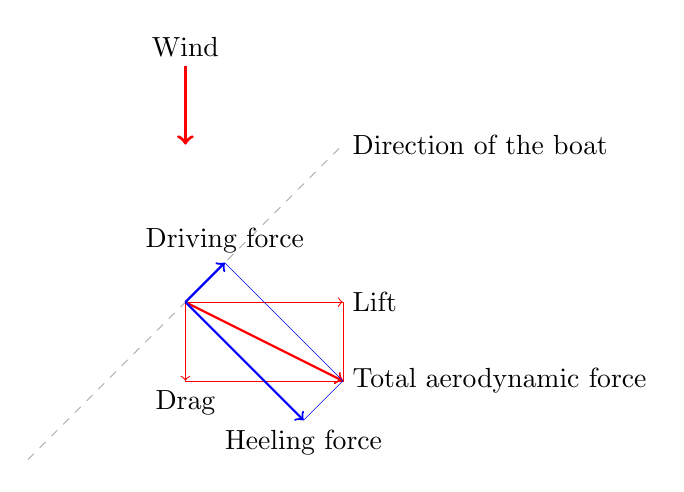
\begin{tikzpicture}
  % keel
  \draw[help lines, dashed] (-2,-2) -- (2,2);

  \node[above, right] at (2,2) {Direction of the boat};
  % wind
  \draw[very thick, red, ->] (0,3) -- (0,2);
  \node[above] at (0,3) {Wind};

  % aerodynamic forces
  \draw[red, ->] (0,0) -- (2,0);
  \draw[red, ->] (0,0) -- (0, -1);
  \draw[thick, red, ->] (0,0) -- (2, -1);
  \draw[help lines, red] (0, -1) -- (2, -1) -- (2, 0);

  \node[right] at (2, 0) {Lift};
  \node[below] at (0, -1) {Drag};
  \node[below, right] at (2, -1) {Total aerodynamic force};

  % hydrodynamic forces
  \draw[blue, thick, ->] (0,0) -- (intersection cs:
  first line={(0,0) -- (3, -3)},
  second line={(2, -1) -- (1, -2)}) coordinate (A);

  \draw[blue, thick, ->] (0,0) -- (intersection cs:
  first line={(0,0) -- (3, 3)},
  second line={(2, -1) -- (1, 0)}) coordinate (B);

  \draw[help lines, blue] (B) -- (2, -1) -- (A);

  \node[right, below] at (A) {Heeling force};
  \node[right, above] at (B) {Driving force};

\end{tikzpicture}

Nice summary of the forces involved
\href{http://grizzly.colorado.edu/~rmw/files/papers/PhysicsofSailing.pdf}{here}.

\begin{itemize}
\item The aerodynamic lift force (\overrightarrow{L}) is perpendicular to the
  wind.
\item The aerodynamic drag force (\overrightarrow{D}) goes in the direction of
  the wind.
\item The normal force (N) is perpendicular to the sail.
\item The axial force (A) is parallel to the sail.
\item The total aerodynamic force is the sum of lift and drag
  $\overrightarrow{F}_T = \overrightarrow{L} + \overrightarrow{D}$.
\item The driving force ($\overrightarrow{F}_R$) goes parallel to the point of
  sail.
\item The heeling force ($\overrightarrow{F}_H$) goes perpendicular to the point
  of sail.
\item Hydrodynamic side force ($\overrightarrow{F}_S$) is the ``lift'' generated
  by the keel against the water. It goes perpendicular to the apparent motion of
  water.
\item The hydrodynamic drag force (\overrightarrow{D}) goes parallel to the
  keel.
\item The total hydrodynamic force is $\overrightarrow{R}_T =
  \overrightarrow{F}_S + \overrightarrow{R}$.
\end{itemize}

I suspect that the drag force, being constrained by the hull, is what produces
the reaction force that pushes the boat forward.

We assume that lift is generated somehow. A sail that has a small angle to the
wind generates less drag, but also less lift. Play with
\href{https://www.grc.nasa.gov/www/k-12/airplane/foil3.html}{foil simulator}, to
experiment.
\end{document}
